% Full-width teaser in the title block. Source: paper/figures/cvpr_v1/fig01_teaser.pdf (+ .json sidecar with every printed number).
\begin{minipage}{\textwidth}
\centering
\captionsetup{type=figure,hypcap=false}
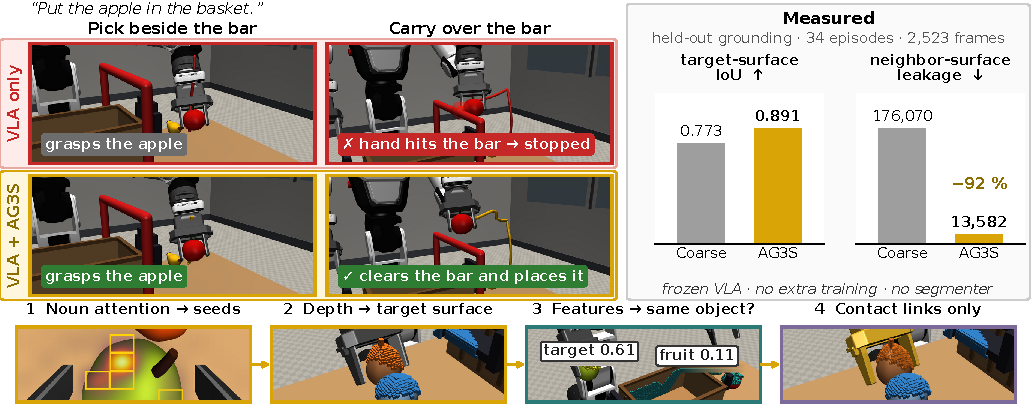
\includegraphics[width=\textwidth]{../figures/cvpr_v1/fig01_teaser_noCL.pdf}
\caption{\textbf{\sys\ lets a frozen VLA touch the object it names, and nothing beside it.}
\emph{Left:} the same policy, scene, seed, and obstacle, recorded on two snapshots of the client. Alone, the policy grasps the apple beside the bar but drives its hand into the bar while carrying and is stopped on contact; with \sys\ it lifts the apple and carries it over. \emph{Bottom}, on a development episode with a pear: noun attention seeds the object, depth continuity recovers its observed surface while the touching fruit stays an obstacle, centered features confirm it is still the same object, and only the designated contact links may enter it (configured rule, illustrated). \emph{Right:} on 34 pre-registered held-out episodes the surface construction improves every episode and, with reassociation, frees \pend{92\%} less neighboring surface than radius growth; closed-loop results are in Tab.~\ref{tab:closedloop}.}
\label{fig:teaser}
\end{minipage}
